% Circumscribed Parallelepiped
% Author: Axel Pavillet
\documentclass[border=10pt]{standalone}
\usepackage{tkz-graph}
\usepackage{relsize}
\usetikzlibrary{arrows,decorations.markings,calc}

\definecolor{cd40000}{RGB}{212,0,0}
\definecolor{cffffff}{RGB}{255,255,255}
\definecolor{c2a7fff}{RGB}{42,127,255}
\definecolor{c0000d9}{RGB}{0,0,217}
\definecolor{c0000ff}{RGB}{0,0,255}

\usepackage{relsize}

\tikzset{every path/.style={draw, ->,>=latex,line width=1pt,color=black}}

%\tikzset{every node/.style={draw,minimum width = 20pt,line width = 1.75pt,
%circle,inner sep=0pt,font = \fontsize{14}{14}\selectfont,fill=none}}

\begin{document}
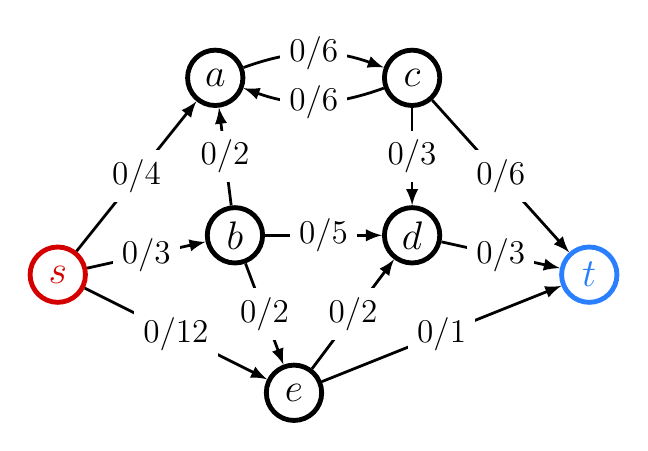
\begin{tikzpicture}[scale=0.5]
\begin{scope}[every node/.style={draw,minimum width = 20pt,line width = 1.75pt,
circle,inner sep=0pt,font = \fontsize{14}{14}\selectfont,fill=none}]
\node[color=cd40000] (s) at (0,3) {$s$};
\node[color=c2a7fff] (t) at (13.5,3) {$t$};
\node (e) at (6,0) {$e$};
\node (a) at (4,8) {$a$};
\node (c) at (9,8) {$c$};
\node (b) at (4.5,4) {$b$};
\node (d) at (9,4) {$d$};
\end{scope}

\path[->] (s) -- (a) node[midway, fill=white, font=\fontsize{12}{12}\selectfont] {$0/4$};
\path[->] (s) -- (b) node[midway, fill=white, font=\fontsize{12}{12}\selectfont] {$0/3$};
\path[->] (s) -- (e) node[midway, fill=white, font=\fontsize{12}{12}\selectfont] {$0/12$};
\path[->] (b) -- (a) node[midway, fill=white, font=\fontsize{12}{12}\selectfont] {$0/2$};
\draw[->] (a) to [bend left=20]  node[midway, fill=white, font=\fontsize{12}{12}\selectfont] {$0/6$} (c);
\draw[->] (c) to [bend left=20]  node[midway, fill=white, font=\fontsize{12}{12}\selectfont] {$0/6$} (a);
\path[->] (b) -- (e) node[midway, fill=white, font=\fontsize{12}{12}\selectfont] {$0/2$};
\path[->] (e) -- (d) node[midway, fill=white, font=\fontsize{12}{12}\selectfont] {$0/2$};
\path[->] (b) -- (d) node[midway, fill=white, font=\fontsize{12}{12}\selectfont] {$0/5$};
\path[->] (d) -- (t) node[midway, fill=white, font=\fontsize{12}{12}\selectfont] {$0/3$};
\path[->] (c) -- (d) node[midway, fill=white, font=\fontsize{12}{12}\selectfont] {$0/3$};
\path[->] (c) -- (t) node[midway, fill=white, font=\fontsize{12}{12}\selectfont] {$0/6$};
\path[->] (e) -- (t) node[midway, fill=white, font=\fontsize{12}{12}\selectfont] {$0/1$};

\end{tikzpicture}
\end{document}